\documentclass[aspectratio=43]{beamer}
\usepackage[utf8]{inputenc}
\usepackage[T1]{fontenc}
\usepackage[english]{babel}
\usepackage{multicol}
\usepackage{listings}
\usepackage{subfigure}
\usepackage{caption}
\usepackage{amsmath,amsthm,amsfonts,amssymb,amscd}
\usepackage[style=verbose,backend=biber,sorting=ynt]{biblatex}
\usepackage{csquotes}
\usepackage{siunitx}
\usepackage{nicefrac}
\usepackage{pifont}% http://ctan.org/pkg/pifont
\newcommand{\cmark}{\ding{51}}%
\newcommand{\xmark}{\ding{55}}%
\frenchspacing

\usetheme{CambridgeUS}
\usecolortheme{rose} %vagy esetleg rose, beaver
\usefonttheme{serif}

\addbibresource{parts/literature.bib}

\beamertemplatenavigationsymbolsempty



% \AtBeginSection[]
% {
%  \begin{frame}<beamer>
%  \frametitle{Plan}
%  \tableofcontents[currentsection]
%  \end{frame}
% }


%címdia
\title[Group Assignment] %optional
{German beers to Hungarian market (webshop)}

\subtitle{}

\author[Marketing]
{Ádám Kohajda \\ Dániel Nagy \\ József Szenka \\ László Kocsis \\ Zoltán Hafner}

\date[April 2022] % (optional)
{April 2022}

\begin{document}

%------------------------Címdia-------------------------------
\begin{frame}[plain]
    \titlepage
\end{frame}

\begin{frame}{Contents}
   \tableofcontents
\end{frame}


%------------------------Bevezetés-------------------------------
\section{Introduction}

\begin{frame}{German beers}
\begin{itemize}
   \item Germany is the largest beer consumer of Europe
   \item 1300 German breweries with more than 110 hectolitre production \footcite{statista1}
   \item German Purity Law
\end{itemize}

\begin{figure}[H]
  \centering
  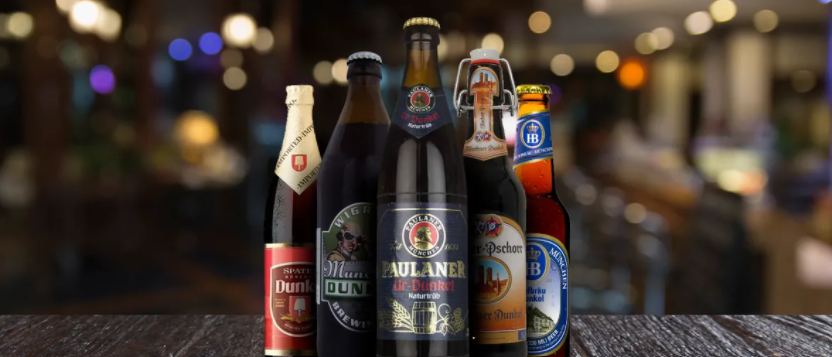
\includegraphics[width=0.6\linewidth]{pics/german_beer.png}
\end{figure}

\end{frame}

\begin{frame}{Hungarian market}
\begin{itemize}
   \item Dynamic transformation in recent years
   \item More and more craft breweries in Hungary
   \item Ride this trend $\rightarrow$ introduce German craft beers
\end{itemize}

\begin{figure}[H]
  \centering
  
\includegraphics[width=0.85\linewidth]{pics/hungarianCraft.jpg}
  \caption*{Hungarian Craftbeer}
\end{figure}

\end{frame}



\section{Analysis}

\subsection{Market segmentation}
\begin{frame}{Geographic segmentation}
   \begin{itemize}
      \item People of villages and rural areas $\rightarrow$ unlikely customers
      \item People of smaller towns $\rightarrow$ some potential customers
      \item People of larger cities and Budapest $\rightarrow$ main base of customers
      \begin{itemize}
         \item Higher income
         \item Around 3.6 million people\footcite{ksh1}
      \end{itemize}
   \end{itemize}

   \begin{figure}[t]
    \centering
    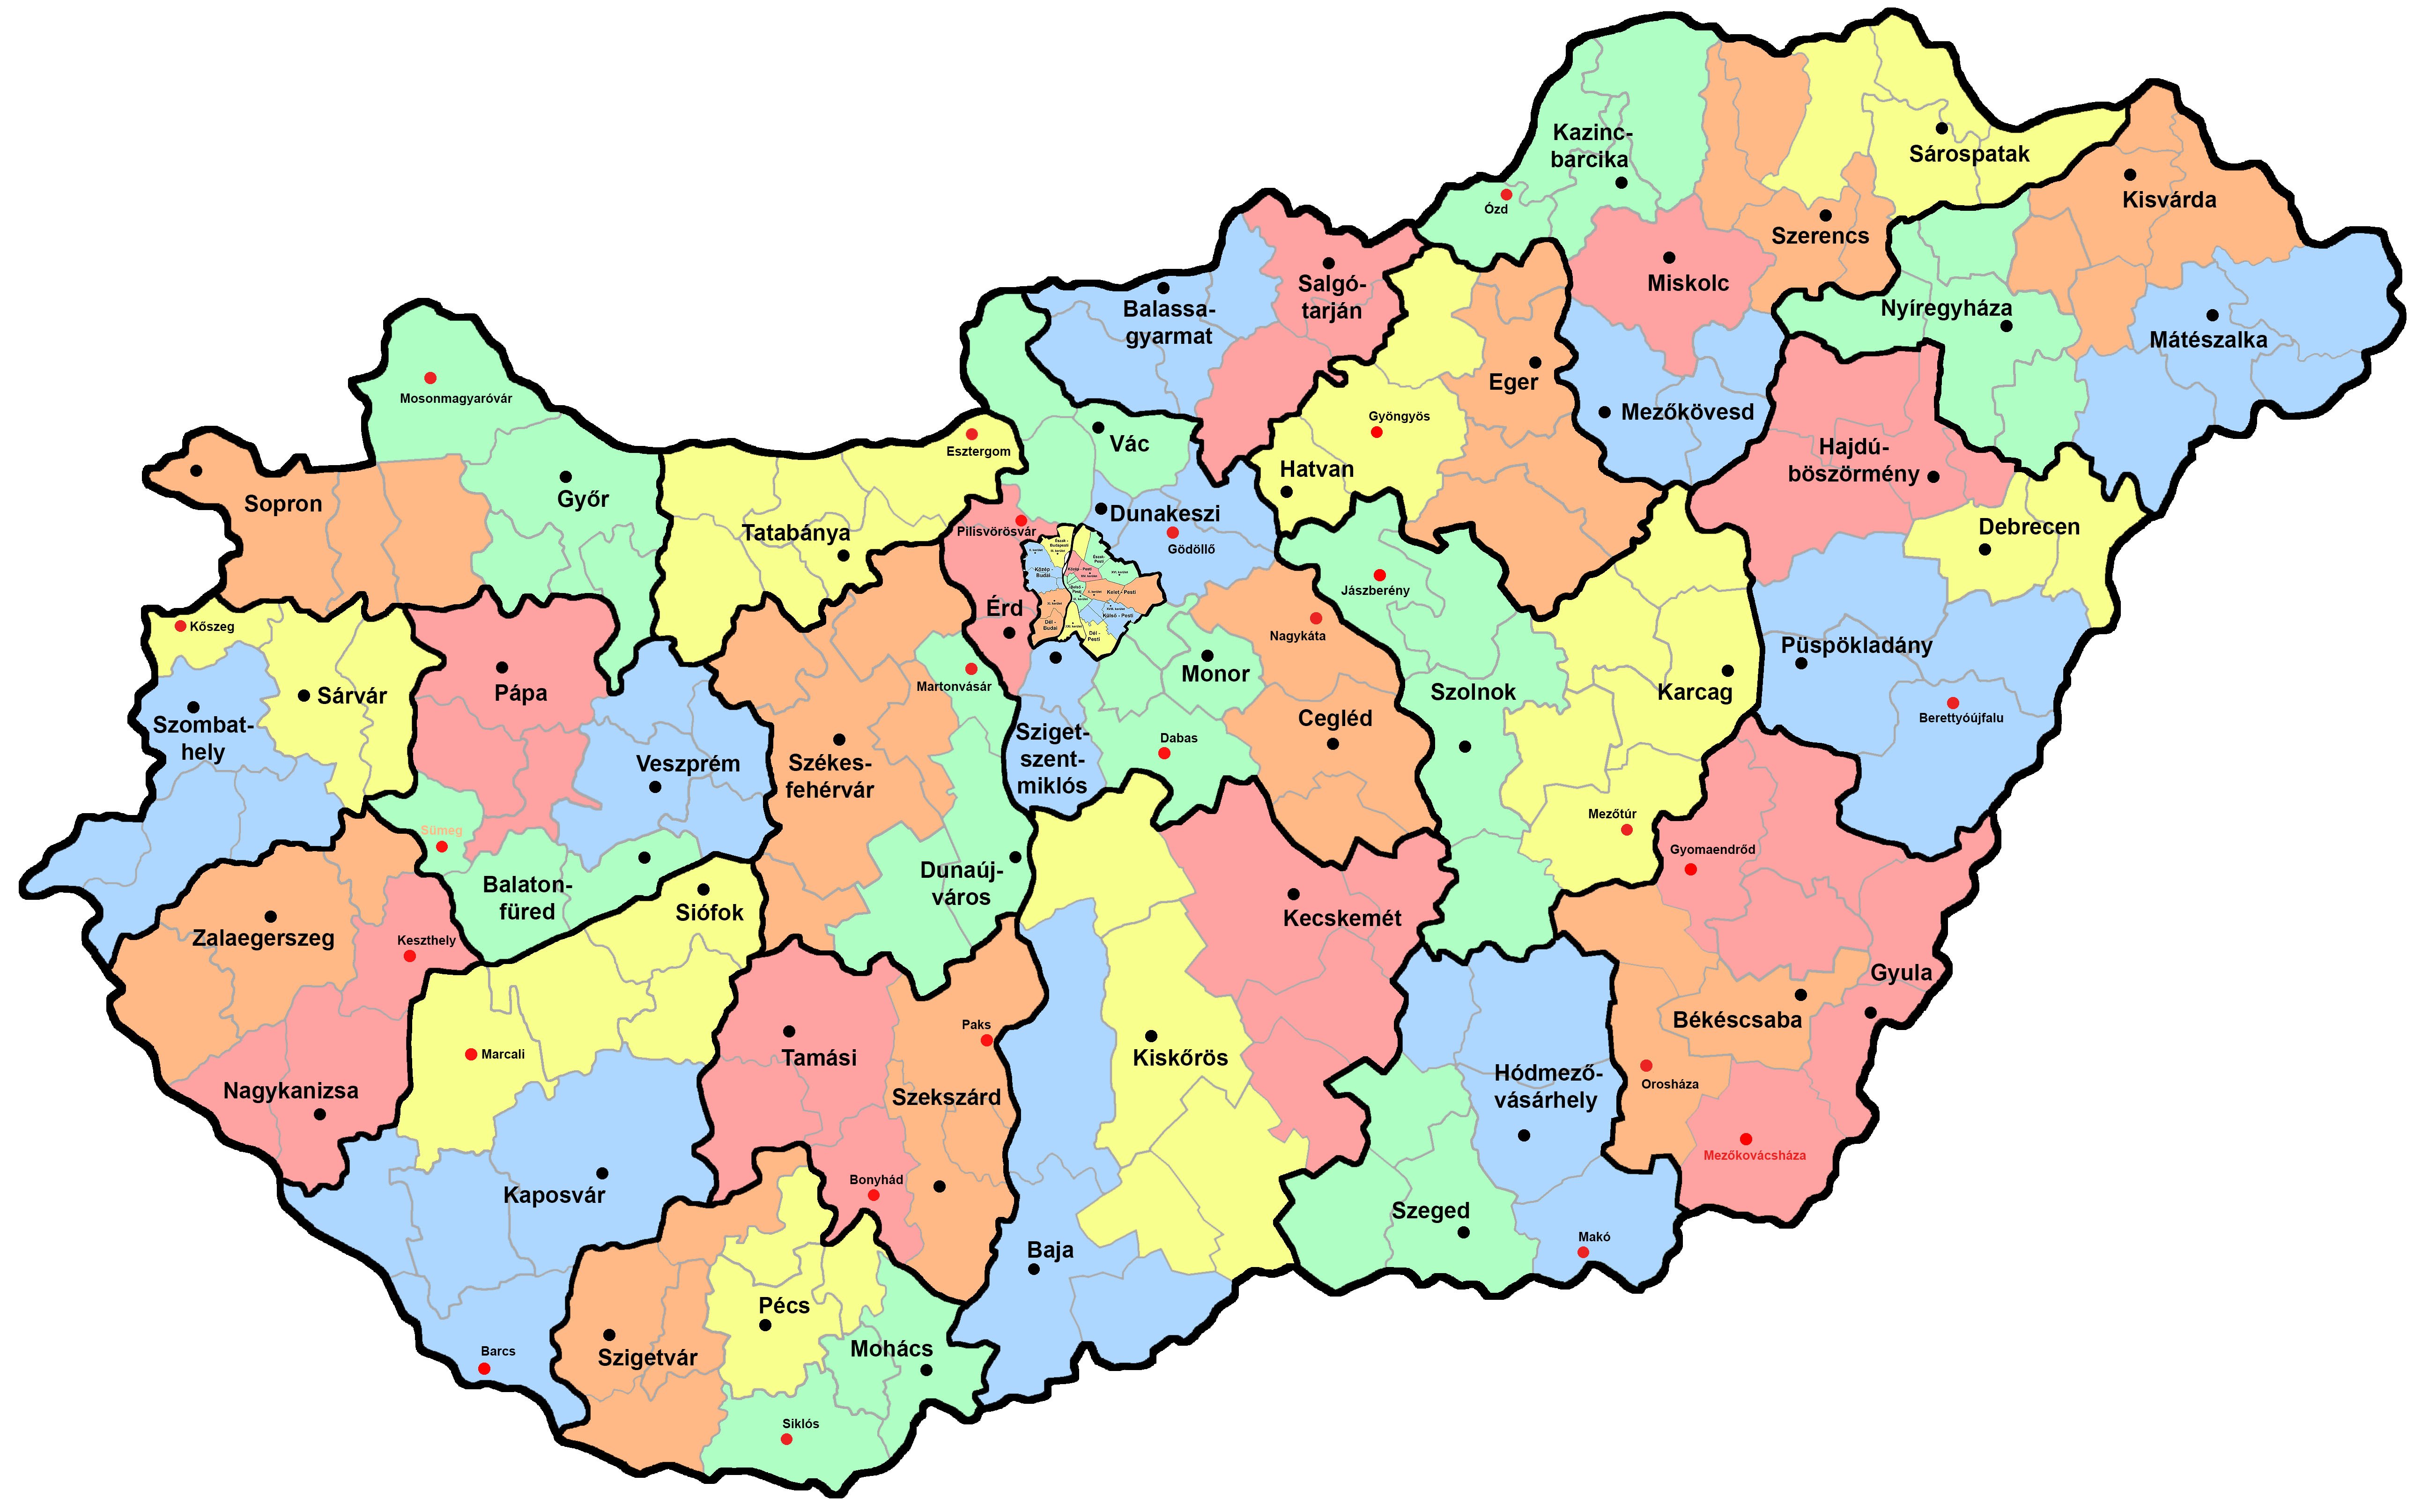
\includegraphics[width=0.45\linewidth]{pics/magyar.jpg}
   \end{figure}
\end{frame}

\begin{frame}{Demographic segmentation}
   \begin{itemize}
      \item 30-60 years men -- most significant beer drinkers \footcite{ksh2}
      \item Younger people -- usually cannot afford quality
   \end{itemize}

   \begin{figure}[H]
     \centering
     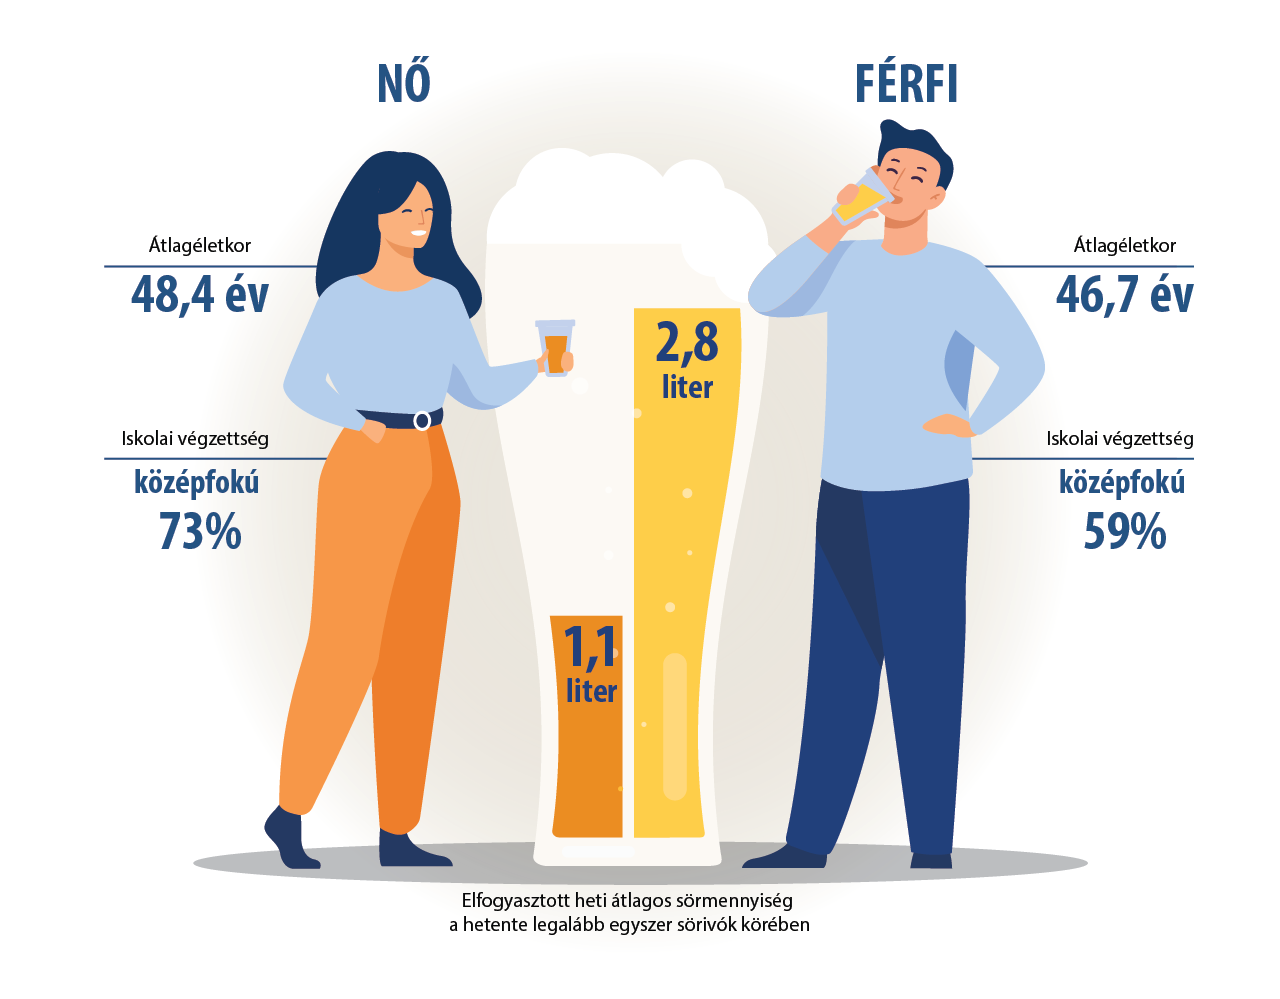
\includegraphics[width=0.45\linewidth]{pics/ksh.png}
     \caption*{Beer consumption behaviour of men and women in Hungary}
   \end{figure}

\end{frame}

\begin{frame}{Psychographic and Behavioral segmentation}
   \begin{itemize}
      \item Men from the middle and upper class
      \item In search of diverse high quality beers
      \item Lifestyle: consume beer rarely (few times a week) but on greater occasions, many of them together with there friends
   \end{itemize}
\end{frame}



\subsection{Market targeting}
\begin{frame}{Targeted Segment}
\begin{itemize}
   \item Middle aged men, living in cities
   \item Stable size
   \item Getting more and more open to imported beers \footcite{ksh2}
\end{itemize}
\begin{figure}[H]
  \centering
  
\includegraphics[width=0.64\linewidth]{pics/bullshit2.png}
\end{figure}
\end{frame}

\begin{frame}{Strategy}
\begin{itemize}
   \item Concentrated marketing strategy
   \item Focus on a single segment
   \item Mainly online marketing
   \item Emphasize high quaity and product diversity
\end{itemize}
\begin{figure}[H]
  \centering
  
\includegraphics[width=0.57\linewidth]{pics/bullshit1.jpg}
\end{figure}
\end{frame}



\subsection{Market positioning}


\begin{frame}{Competitors}

   \begin{columns}
      \begin{column}{0.4\textwidth}
         \begin{itemize}
            \item \texttt{soronline.hu}
            \item \texttt{beerselection.hu}
            \item \texttt{beergourmet.hu}
            \item \texttt{csakajosor.hu}
         \end{itemize}
      \end{column}
      \begin{column}{0.6\textwidth}
         \begin{figure}[H]
           \centering
           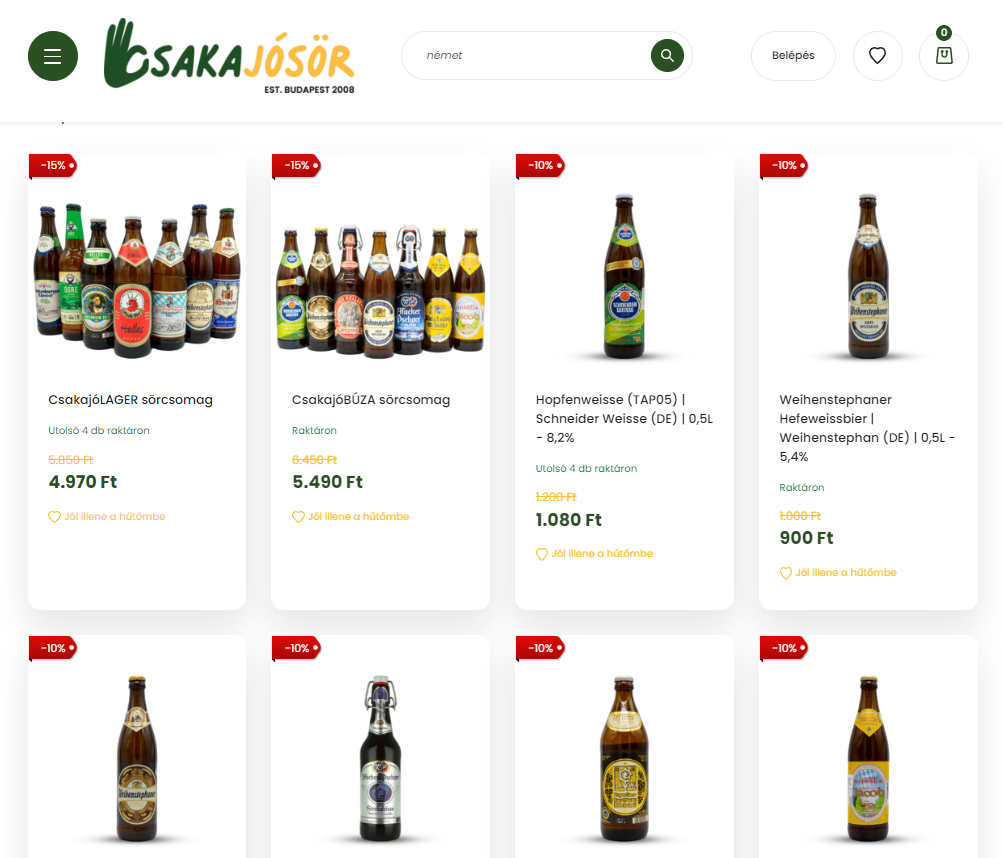
\includegraphics[width=\linewidth]{pics/csakajosor.png}
           \caption*{ \texttt{csakajosor.hu}}
         \end{figure}
      \end{column}
   \end{columns}


\end{frame}

\begin{frame}{Competitive advantage}
\begin{itemize}
   \item Competitors focus on worldwide beer selections $\rightarrow$ only offer a few German beer types
   \item Prioritise German beer types
   \item High quality and the diversity of our product assortment
\end{itemize}
\begin{figure}[H]
  \centering
  
\includegraphics[width=0.57\linewidth]{pics/bullshit3.jpg}
\end{figure}
\end{frame}

\begin{frame}{Positioning statement}

      \textit{To quality beer consumers who enjoy a wide variety of German beers, our webshop is the ultimate place that delivers the perfect beer for your every day consumption as well as for special occasions.}

\end{frame}






\section{Summary}

\begin{frame}{Summary}
\begin{itemize}
   \item Focus on: Middle aged men living in cities
   \item Wealthy enough to afford the quality
   \item Quality of life is increasing in Hungarian cities $\rightarrow$ increased demand
\end{itemize}
\end{frame}


\section{References}
\begin{frame}{References}
   \begin{columns}
      \begin{column}{0.9\textwidth}

         \printbibliography[heading=none]
      \end{column}
   \end{columns}

\end{frame}


\begin{frame}{Thank you for the attention!}
   \begin{figure}[H]
     \centering
     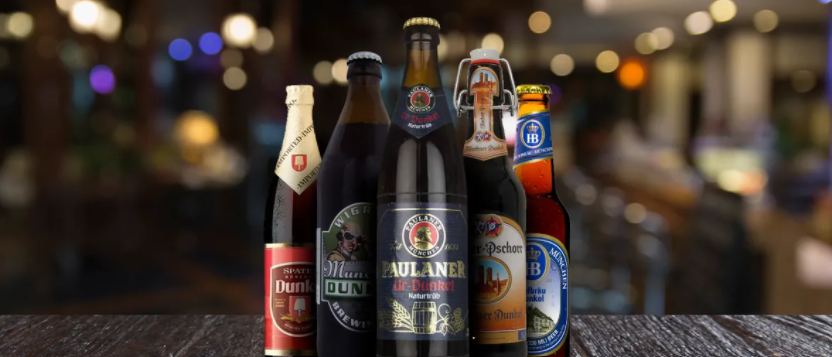
\includegraphics[width=0.9\linewidth]{pics/german_beer.png}
   \end{figure}
\end{frame}




\end{document}
